\documentclass[..thesis.tex]{subfiles}
\tikzset{xyp/.style={canvas is xy plane at z=#1}}
\tikzset{xzp/.style={canvas is xz plane at y=#1}}
\tikzset{yzp/.style={canvas is yz plane at x=#1}}

\pgfmathsetmacro{\cubex}{5}
\pgfmathsetmacro{\cubey}{5}
\pgfmathsetmacro{\cubez}{5}

\newcommand{\opacity}{0.8}

% 1 - x_1, 2 - y_1, 3 - z_1, 4 - x_2, 5 - y_2, 6 - z_2, 7 - color
\newcommand{\drawcube}[7]
{
      \filldraw[opacity=\opacity, #7, draw=black, dashed, xzp=#2] (#1,#3) rectangle (#4,#6);
      \filldraw[opacity=\opacity, #7, draw=black, dashed, xzp=#5] (#1,#3) rectangle (#4,#6);
      \filldraw[opacity=\opacity, #7, draw=black, dashed, xyp=#3] (#1,#2) rectangle (#4,#5);
      \filldraw[opacity=\opacity, #7, draw=black, dashed, xyp=#6] (#1,#2) rectangle (#4,#5);
      % not drawing left side intentionally
      \filldraw[opacity=\opacity, #7, draw=black, dashed, yzp=#4] (#2,#3) rectangle (#5,#6);
}

\newcommand{\drawcubeoverz}[5]
{
 \drawcube{#1}{#2}{0}{#3}{#4}{\cubez}{#5}
}

\newcommand{\drawoutercube}
{
      \draw[thick,-] (0,0,0) -- ++(\cubex,0,0) -- ++(0,0,\cubez) -- node [anchor = north] {$B$} ++(-0.5*\cubex,0,0) --  node [anchor = north] {$A$} ++(-0.5*\cubex,0,0)  --   ++(0,0,-\cubez);
      \draw[thick,-] (0,\cubey,0) -- ++(\cubex,0,0) -- ++(0,0,\cubez) -- ++(-\cubex,0,0) --   ++(0,0,-\cubez)  ;

      \draw[thick,-] (0,0,0) -- (0,\cubey,0);
      \draw[thick,-] (\cubex,0,0) -- (\cubex,\cubey,0);
      \draw[thick,-] (\cubex,0,\cubez) -- ++(0,\cubey,0);
      \draw[thick,-] (0,0,\cubez) -- (0,\cubey,\cubez);
}

%%%%%%% Colors %%%%%%

\newcommand{\defaultPColor}{yellow}
\newcommand{\defaultPLColor}{\defaultPColor!50}
\newcommand{\defaultPRColor}{\defaultPColor!75}

\newcommand{\aColor}{blue}
\newcommand{\aLColor}{\aColor!30}
\newcommand{\aRColor}{\aColor!75}

\newcommand{\bColor}{green}
\newcommand{\bLColor}{\bColor!50}
\newcommand{\bRColor}{\bColor!95}
      
\newcommand{\bIColor}{purple}
\newcommand{\bILColor}{\bIColor!30}
\newcommand{\bIRColor}{\bIColor!95}

\newcommand{\defaultColor}{red}
\newcommand{\defaultLColor}{\defaultColor!30}
\newcommand{\defaultRColor}{\defaultColor!75}

\newcommand{\initColor}{red}
\newcommand{\initLColor}{\initColor!30}
\newcommand{\initRColor}{\initColor!75}

\newcommand{\postInitColor}{blue}
\newcommand{\postInitLColor}{\postInitColor!30}
\newcommand{\postInitRColor}{\postInitColor!75}

\begin{document}

The key challenge for static analyzers based on abstract interpretation is to minimize the loss of precision that inevitably accompanies the over-approximation.
In case of analyses trying to detect data-races, the loss of precision casuse static analysers to emit false-positives and it is clear
that even if one can guarantee the soundness of the underlying analysis,
then there is a threshold of incorrect warnings above what the results of the analysis contain too much noise to be of help for the end user.

We will now introduce two analyses that, when combined with other analyses, help to increase the precision of a static analyzer that detects data-races. Both of these analyses are implemented in static analyzer \textit{Goblint}, that we will discuss further in the next section.

\toadd{Check that Goblint is mentioned in next section}

\toguide{Okay, what is the point of it?}

\subsection{Region Analysis}

First of those is the \textit{region analysis}. The key idea behind this analyses is to try to partition the memory used by the program under analyses into disjoint regions -- based on this information we can deduce that memory accesses to different regions cannot data-race.

Consider a hash table using chaining to handle hash collisions that has a lock for each of the buckets.

\begin{figure}[H]
  \centering
  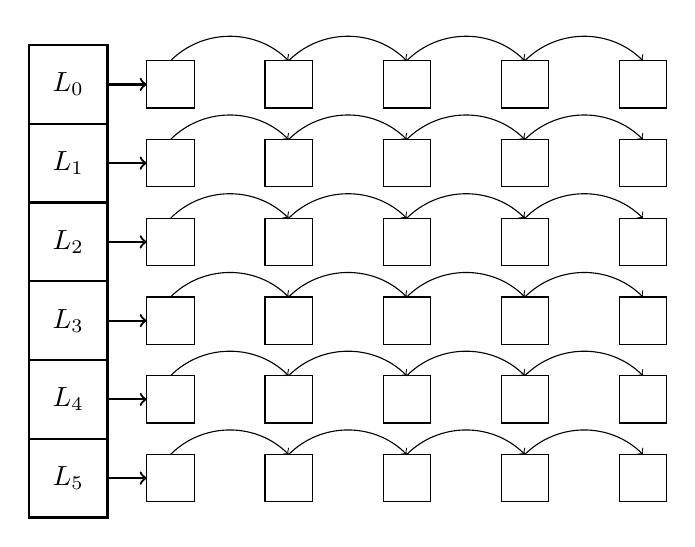
\begin{tikzpicture}
    \foreach \y in {0,...,5}
      {
        \draw[thick]  (0,5 - \y) rectangle  ++(1,1) node[midway] {$L_{\y}$};
        \draw[->, thick] (1,5 - \y + 0.5) -- ++(0.5,0);
        \foreach \x in {1,...,5}
        {
          \draw (1.5*\x, 5 -\y+0.2) rectangle ++(0.6,0.6);

        }
        \foreach \x in {1,...,4}
        {
          \draw[->] (1.5*\x + 0.3, 5 - \y + 0.8) to [bend left=45] ++(1.5,0);
        }
      }
  \end{tikzpicture}
  \caption{Separate chaining hash table} 
\end{figure}

An usual way to synchronize such an hash table is to protect each bucket with its own lock --
if the hashes of the keys $k_1$ and $k_2$ are different then accessing them in the hash table cannot cause a data race.
On the other hand, if $k_1$ and $k_3$ produce the same hash then there is a real risk for data race.


\begin{figure}[H]
  \centering
  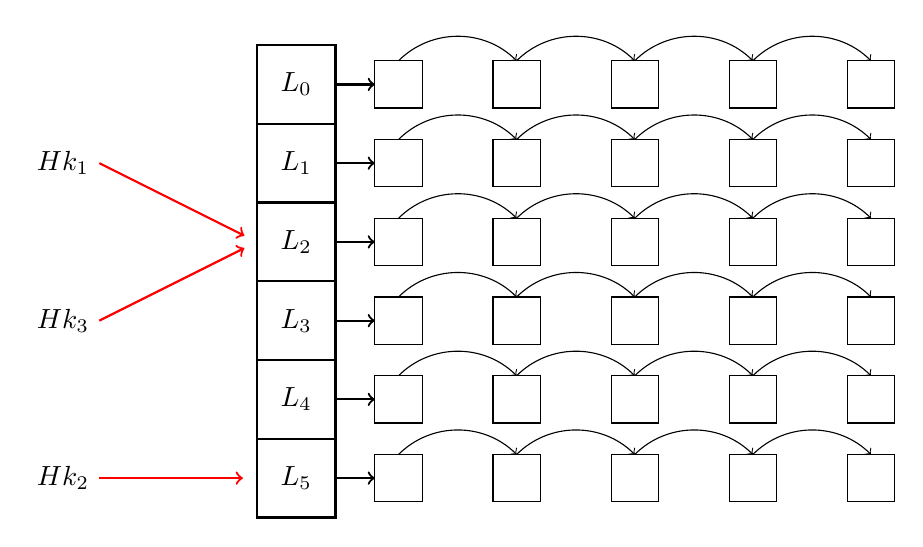
\begin{tikzpicture}
    \foreach \y in {0,...,5}
      {
        \draw[thick]  (0,5 - \y) rectangle  ++(1,1) node[midway] {$L_{\y}$};
        \draw[->, thick] (1,5 - \y + 0.5) -- ++(0.5,0);
        \foreach \x in {1,...,5}
        {
          \draw (1.5*\x, 5 -\y+0.2) rectangle ++(0.6,0.6);

        }
        \foreach \x in {1,...,4}
        {
          \draw[->] (1.5*\x + 0.3, 5 - \y + 0.8) to [bend left=45] ++(1.5,0);
        }
      }
    \draw[red, ->, shorten >= 5pt, thick] (-2,2.5) node [black, anchor =  east] {$H\lp k_3 \rp$} -- (0,3.5);
    \draw[red, ->, shorten >= 5pt, thick] (-2,0.5) node [black, anchor =  east] {$H\lp k_2 \rp$} -- (0,0.5); 
    \draw[red, ->, shorten >= 5pt, thick] (-2,4.5) node [black, anchor =  east] {$H\lp k_1 \rp$} -- (0,3.5);
      
  \end{tikzpicture}
  \caption{Separate chaining hash table} 
\end{figure}


If we can guarantee that when adding an element for key $k_1$ and for key $k_3$, we are accessing different regions of the memory, then we can deduce that these additions cannot cause a data race.

In case of the hash table, the most obvious partition for the regions would be to separate the buckets of the hash table.


\begin{figure}[H]
  \centering
    \begin{tikzpicture}
      \pgfmathsetmacro{\cubex}{10}

      
      \tikzset{xzp/.style={canvas is xz plane at y=#1}}


      \foreach \x in {1,...,5} 
      {
        \draw[thick,dashed] (\x*\cubex*0.2,0,0) -- ++(0,0,\cubez);
      }

      \fill[opacity=0.8,red!30,draw=black,xzp=0] (0,0) rectangle (0.2*\cubex,\cubez);
      \fill[opacity=0.8,blue!40,draw=black,xzp=0] (0.2*\cubex,0) rectangle (0.4*\cubex,\cubez);
      \fill[opacity=0.8,green!40,draw=black,xzp=0] (0.4*\cubex,0) rectangle (0.6*\cubex,\cubez);
      \fill[opacity=0.8,yellow!50!red,draw=black,xzp=0] (0.6*\cubex,0) rectangle (0.8*\cubex,\cubez);
      \fill[opacity=0.8,cyan!40,draw=black,xzp=0] (0.8*\cubex,0) rectangle (\cubex,\cubez);

      \node at (0.275*\cubex,0,0.4*\cubez) (p) {$H \lp k_1 \rp$};
      \node at (0.3*\cubex,0,0.75*\cubez) (q) {$H \lp k_3 \rp$};

      \node at (0.9*\cubex,0,0.35*\cubez) (q) {$H \lp k_2 \rp$};


      \draw[thick,-] (0,0,0)  -- ++(0,0,\cubez) --  node [anchor = north] {$R_1$} ++(0.2*\cubex,0,0) -- node [anchor = north] {$R_2$} ++(0.2*\cubex,0,0) -- node [anchor = north] {$R_3$} ++(0.2*\cubex,0,0) -- node [anchor = north] {$R_4$} ++(0.2*\cubex,0,0) -- node [anchor = north] {$R_5$} ++(0.2*\cubex,0,0)  --  ++(0,0,-\cubez) -- ++(-\cubex,0,0);
    \end{tikzpicture}
    \caption{Memory partition of the hash table}
\end{figure}

More information regarding region analysis can be found in \cite[66]{vojdanivesal_static_2010}.

\subsection{Region analysis for time}

In addition to device drivers containing disjoint regions of memory, there are also disjoint time intervals.

\toguide{How can you use happen-before here?}

Consider following simplified device driver:

\begin{lstlisting}[language=c,style=def]

static int i = 0;
static int j = 0;

static int file_open(file* f, ...)
{
    printk( "Opening device \n");
    file -> private_data += 1;
    j += 1;
    return 0;
}

static int file_close(file* f, ...)
{
    printk( "Closing device \n");
    file -> private_data -= 1
    j -= 1;
    return 0;
}

int a(file f, ...)
{
  j += 1;
  return 0;
}

int b(file f, ...)
{
  j += 1
  return 0;
}

struct file_operations f_ops = {
  .open    = file_open,
  .release = file_close,
};

int init(...)
{
  publish_file_operations(f_ops);
  i += 1;
  return 0;
}

int exit(...)
{
  i -= 1;
  return 0;
}

\end{lstlisting}

As mentioned previously, \inlinecode{init} and \inlinecode{exit} functions are used by kernel register and deregister a device.
As after publishing the file operations, we cannot any longer assume that the functions of the driver are called by one thread and
a possible data-race should be detected between the operations on variable $i$ in functions \inlinecode{init} and \inlinecode{exit} by a static analyzer that detects data races.
At same time, the Linux Kernel does not allow a call to the \inlinecode{exit} function until the call to the \inlinecode{init} function is called and all the opened files are released.

We would like to have an analysis that knows about such guarantees and can make use of the information that they provide.

\toguide{Example makes sense, but how to practically make use of it?}

To do so, inspired by the happens-before relation,  we extend the region analysis to cover time in addition to space.

\toguide{Erghh, was not the easiest part of the Goblint section. A bit of refreshment would be great.}
\tosup{I am now even more convinced that you should have a chapter on ``Region Analysis for Space and Time'' where you first describe the current region analysis and extend it with timed partitions. Then, you have a section with just implementation. The only question is where to put any experimental results.}

For example, let us have two procedures , \inlinecode{f} and \inlinecode{g} that can be ran simultaneously in different threads.

\begin{lstlisting}[language=c,style=def]

int* p;
int* q;

void f()
{
  &p = &q - 1; 
}

void g()
{
  &q = &q + 1; 
}

\end{lstlisting}

 

If we can divide the memory used by the program to two regions, $A$ and $B$ that are disjoint and we can guarantee that the pointer \inlinecode{p} points
to integer variable stored in region $A$ and \inlinecode{q} points to integer variable stored in region $B$ then we can safely assume that there
can be no data-race between the increment and decrement operations in function \inlinecode{f} and \inlinecode{g}. This can be done by the region analysis.

\begin{figure}[H]
  \centering
    \begin{tikzpicture}
      \draw[thick,-] (0,0,0)  -- ++(0,0,\cubez) --  node [anchor = north] {$A$} ++(0.5*\cubex,0,0) -- node [anchor = north] {$B$} ++(0.5*\cubex,0,0)   --  ++(0,0,-\cubez) -- ++(-\cubex,0,0);
      \draw[thick,dashed] (0.5*\cubex,0,0) -- ++(0,0,\cubez);
      \fill[opacity=\opacity,red!30,draw=black,xzp=0] (0,0) rectangle (2.5,5);
      \fill[opacity=\opacity,red!75,draw=black,xzp=0] (2.5,0) rectangle (5,5);

      \node at (0.15*\cubex,0,0.6*\cubez) (p) {\figcode{\&p}};
      \node at (0.8*\cubex,0,0.75*\cubez) (q) {\figcode{\&q}};

      \node at (0.35*\cubex,0,0.35*\cubez) (q) {\figcode{i}};
    \end{tikzpicture}
    \caption{Memory partition as done by region analyses}
\end{figure}

Going back to the example driver, this does allow to eliminate the data race between the assignments to \inlinecode{i} in \inlinecode{init} and \inlinecode{exit} functions.
However, if we would enhance the region analysis with one more dimension that would roughly correspond to time,
we could divide the memory as seen on the following illustration. 

\begin{figure}[H]
  \centering
    \begin{tikzpicture}

      \drawcubeoverz{0}{0}{0.5*\cubex}{0.5*\cubey}{\initLColor}
      
      \drawcubeoverz{0}{0.5*\cubey}{0.5*\cubex}{\cubey}{\postInitLColor}

      \drawcubeoverz{0.5*\cubex}{0}{\cubex}{0.5*\cubey}{\initRColor}      

      \drawcubeoverz{0.5*\cubex}{0.5*\cubey}{\cubex}{\cubey}{\postInitRColor}

      \drawoutercube

      \node at (0.285*\cubex,0.15*\cubey,0.7*\cubez) (ip) {\figsubcode{i}{init}};
      \node at (0.285*\cubex,0.8*\cubey,0.7*\cubez) (i) {\figsubcode{i}{exit}};

      \draw[thick,-] (0,0,\cubez) -- node[anchor= east] {$init$} ++(0,0.5*\cubey,0)  -- node[anchor= east] {$postInit$}  ++(0,0.5*\cubey,0);
    \end{tikzpicture}
    \caption{Memory partition with addition of time dimension}
\end{figure}

This would let us exclude the possibility of race between these two operations. 

\toguide{How is it done?}

To do this, we would need to track information for each read and write operation.

\toask{\sout{operation bad word?}}
\toask{Should this be moved to region analyses? Seems like a better fit as it originates from there, just using it in timed region analyses. The downside of that would be that I would have to rework the examples (or leave example and introduction far apart, what I have tried to avoid)?}

We will divide the information tracked into \textit{left} and \textit{right} side. 

On the left side, information regarding the memory region of the variable is stored as a set of sets, $C$,
 such that every element of $C$, $I$ describes an intersection of memory regions.

In our example driver, the $C$ for the increment operation on $i$ in the $init$ function would be 

\begin{equation*}
\lb \lb A, init \rb \rb \text{.}
\end{equation*} 

On the right side, information regarding possible reasons why data race cannot take place with another read or write operation is stored in a set $M$.
For an example, $M$ could contain the set of locks held at the specific operation or whether or not the thread running the procedure containing the operation is guaranteed to be unique.

When deciding if there is a possibility of a data race between operations $a$ and $b$, we use two predicates, $L$ and $R$ to evaluate left and right sides of these operations. 

The first of those predicates is defined as follows

\begin{equation*}
L \lp C_a, C_b \rp =  C_a \cap C_b \neq \emptyset \text{.}
\end{equation*}

If $L \lp C_a, C_b \rp$ evaluates to false it means that the two operations do not share a common memory region and hence there cannot be a data race. 

The second predicate, $R$ evaluates the sets $M_a$ and $M_b$ and returns true if there is something that guarantees that the operations $a$ and $b$ cannot race.
 For example, it could be when performing both of these operations, lock $l$ must be held or in case of $a=b$,
 there is a guarantee that there can be only one thread running that executes the operation.

Equipped with those definitions, we can guarantee that operations $a$ and $b$ cannot race if the implication

\begin{equation}
\label{implication}
L \lp C_a, C_b \rp \implies R \lp M_a, M_b \rp  
\end{equation}

holds.

Coming back to our example driver, one can see that using the enhanced region analyses, we can now see that there cannot be a race between $i_{init}$ and $i_{exit}$.
Indeed, as

\toask{Or should we take A as a set of regions, i.e instead of $\lb A, init \rb $ have $C_A \cup \lb init \rb$ ? Would be more correct, but increases complexity?}

\begin{equation*}
 \lb \lb A, init \rb \rb \cap  \lb \lb A, postInit \rb \rb = \emptyset
\end{equation*}

then $L \lp C_{i_{init}}, C_{i_{postInit}} \rp$ is false and the implication (\ref{implication}) holds for $i_{init}$ and $i_{exit}$.

As an example of right hand sides excluding an data race, if we take both $a$ and $b$ to be $i_{init}$ then when evaluating 

\begin{equation*}
R \lp M_{i_{init}}, M_{i_{init}} \rp
\end{equation*} 

we can take into account that Linux kernel does not allow one to register the same driver more than once and as such,
we can guarantee that the thread running the $init$ function is unique.

Based on that information $R \lp M_{i_{init}}, M_{i_{init}} \rp$ holds and so does the implication (\ref{implication}).

\toguide{Does this thing scale, anything else you can do other than init/exit?}

One might have noticed that our example drivers has two extra function, $a$ and $b$. Lets now suppose that similar property holds for $a$ and $b$ --
during the lifetime of driver, we can only call $a$ once and $b$ once and call to $a$  must happen before call to $b$.

Let this be the regions of the program, enhanced with the extra dimension, taking into account only the division by $a$ and $b$:

%%%%%%%%%%%%%%%%%%%%% Height values for a and b %%%%%%%%%%%%%%%%%%%%

 \pgfmathsetmacro{\defaultH}{0.2}
 \pgfmathsetmacro{\aH}{0.45}
 \pgfmathsetmacro{\bH}{0.8}

%%%%%%%%%%%%%%%%%%%%%%%%%%%%%%%%%%%%%%%%%%%%%%%%%%%%%%%%%%%%%%%%%%%%

\begin{figure}[H]
  \centering
    \begin{tikzpicture}
      
      \drawcubeoverz{0}{0}{0.5*\cubex}{\defaultH*\cubey}{\defaultLColor}

      \drawcubeoverz{0}{\defaultH*\cubey}{0.5*\cubex}{\aH*\cubey}{\aLColor}

      \drawcubeoverz{0}{\aH*\cubey}{0.5*\cubex}{\bH*\cubey}{\bLColor}

      \drawcubeoverz{0}{\bH*\cubey}{0.5*\cubex}{\cubey}{\defaultLColor}

      \drawcubeoverz{0.5*\cubex}{0}{\cubex}{\defaultH*\cubey}{\defaultRColor}

      \drawcubeoverz{0.5*\cubex}{\defaultH*\cubey}{\cubex}{\aH*\cubey}{\aRColor}

      \drawcubeoverz{0.5*\cubex}{\aH*\cubey}{\cubex}{\bH*\cubey}{\bRColor}

      \drawcubeoverz{0.5*\cubex}{\bH*\cubey}{\cubex}{\cubey}{\defaultRColor}

      \drawoutercube

      
      \node at (0.65*\cubex,0.1*\cubey,0.4*\cubez) (ip) {\figsubcode{j}{a}};
      \node at (0.65*\cubex,0.5*\cubey,0.4*\cubez) (i) {\figsubcode{j}{b}};

      \draw[thick,-] (0,0,\cubez) -- node[anchor= east] {$default$} (0,\defaultH*\cubey,\cubez) -- node[anchor= east] {$a$}  (0,\defaultH*\cubey,\cubez)  --
      node[anchor= east] {$b$}  (0,\bH*\cubey,\cubez) -- node[anchor= east] {$default$}  (0,\cubey,\cubez);


    \end{tikzpicture}
    \caption{Memory partition with addition of time dimension by $a$ and $b$}
\end{figure}

If we want to combine this time division with the one we could find the Cartesian product of the two and use that as demonstrated on the next figure.

\begin{figure}[H]
  \centering
    \begin{tikzpicture}

      \drawcubeoverz{0}{0}{0.5*\cubex}{\defaultH*\cubey}{\defaultLColor}

      \drawcubeoverz{0}{\defaultH*\cubey}{0.5*\cubex}{\aH*\cubey}{\aLColor}

      \drawcubeoverz{0}{\aH*\cubey}{0.5*\cubex}{0.5*\cubey}{\bILColor}

      \drawcubeoverz{0}{0.5*\cubey}{0.5*\cubex}{\bH*\cubey}{\bLColor}

      \drawcubeoverz{0}{\bH*\cubey}{0.5*\cubex}{\cubey}{\defaultPLColor}

      \drawcubeoverz{0.5*\cubex}{0}{\cubex}{\defaultH*\cubey}{\defaultRColor}

      \drawcubeoverz{0.5*\cubex}{\defaultH*\cubey}{\cubex}{\aH*\cubey}{\aRColor}

      \drawcubeoverz{0.5*\cubex}{\aH*\cubey}{\cubex}{0.5*\cubey}{\bIRColor}

      \drawcubeoverz{0.5*\cubex}{0.5*\cubey}{\cubex}{\bH*\cubey}{\bRColor}
      
      \drawcubeoverz{0.5*\cubex}{\bH*\cubey}{\cubex}{\cubey}{\defaultPRColor}

      
      \node at (0.65*\cubex,0.1*\cubey,0.4*\cubez) (ip) {\figsubcode{j}{a}};
      \node at (0.65*\cubex,0.5*\cubey,0.4*\cubez) (i) {\figsubcode{j}{b}};

      \node at (0.285*\cubex,0.2*\cubey,0.65*\cubez) (ip) {\figsubcode{i}{init}};
      \node at (0.285*\cubex,0.8*\cubey,0.65*\cubez) (i) {\figsubcode{i}{exit}};

      \drawoutercube

      \draw[thick,-] (0,0,\cubez) -- node[anchor= east] {$default \land init$} (0,\defaultH*\cubey,\cubez) -- node[anchor= east] {$a \land init$}  (0,\aH*\cubey,\cubez) 
      -- node[anchor= east] {$b \land init$}  (0,0.5*\cubey,\cubez)-- node[anchor= east] {$b \land postInit$}  (0,\bH*\cubey,\cubez) --
      node[anchor= east] {$default \land postInit$}  (0,\cubey,\cubez);


    \end{tikzpicture}
    \caption{Memory partition with addition of combined time dimension}
\end{figure}

Here, the set $C$ for the increment operation of $i$ in the $init$ function would be

\begin{equation*}
\lb \lb A, init, default \rb, \lb A, init, a \rb, \lb A, init, b \rb \rb
\end{equation*}

and for the decrement operation of $j$ in $b$ it would be

\begin{equation*}
\lb \lb B, init, b \rb, \lb B, postInit, b \rb \rb \text{.}
\end{equation*}

\toguide{Wait, this does not really scale, does it?}

It is easy to see that this approach does not scale too well -- in the worst case the computational difficulty will grow exponentially with added time partition.

\toask{Memory region?}

However, lets notice that when we evaluate the left sides of two operations, the time dimension only has an effect if memory regions of the operations match. 

Indeed, let $Mem$ be the set of all memory regions, let \inlinesubcode{i}{a} and \inlinesubcode{i}{b} be two operations with left sides $C_{i_{a}}$ and $C_{i_{b}}$ such that they do not share a common memory region,
that is

\begin{equation*}
\forall \lp c_1, c_2 \rp, c_1 \in C_{i_a} , c_2 \in C_{i_b} , \lnot \lp \exists m \in Mem,  m \in c_1 \land m \in c_2 \rp
\end{equation*} 

\toask{Should require this somewhere?}

and as at same time, all the entries of the left hand side must contain a memory region then it is clear that $C_{i_{a}} \cap C_{i_{b}} = \emptyset$ and by definition,
$\lnot L \lp C_{i_{a}}, C_{i_{b}} \rp $. 

With that in mind, then for the time partition of memory region $A$ we can take Cartesian product off all the time partitions that effect an operation located in region $A$.
For our running example, the partition would look as follows:

\begin{figure}[H]
  \centering
    \begin{tikzpicture}

      \drawcubeoverz{0}{0}{0.5*\cubex}{0.5*\cubey}{cyan!40}
      
      \drawcubeoverz{0}{0.5*\cubey}{0.5*\cubex}{\cubey}{yellow!50!red}

      \drawcubeoverz{0.5*\cubex}{0}{\cubex}{\defaultH*\cubey}{\defaultRColor}

      \drawcubeoverz{0.5*\cubex}{\defaultH*\cubey}{\cubex}{\aH*\cubey}{\aRColor}

      \drawcubeoverz{0.5*\cubex}{\aH*\cubey}{\cubex}{\bH*\cubey}{\bRColor}

      \drawcubeoverz{0.5*\cubex}{\bH*\cubey}{\cubex}{\cubey}{\defaultPRColor}
      
      \node at (0.65*\cubex,0.1*\cubey,0.4*\cubez) (ip) {\figsubcode{j}{a}};
      \node at (0.65*\cubex,0.5*\cubey,0.4*\cubez) (i) {\figsubcode{j}{b}};

      \node at (0.285*\cubex,0.2*\cubey,0.65*\cubez) (ip) {\figsubcode{i}{init}};
      \node at (0.285*\cubex,0.8*\cubey,0.65*\cubez) (i) {\figsubcode{i}{exit}};

      \drawoutercube

      
      \draw[thick,-] (0,0,\cubez) -- node[anchor= east] {$init$} ++(0,0.5*\cubey,0)  -- node[anchor= east] {$postInit$}  ++(0,0.5*\cubey,0);
      \draw[thick,-] (\cubex,0,0) -- node[anchor= west] {$default$} (\cubex,\defaultH*\cubey,0) -- node[anchor= west] {$a$}  (\cubex,\aH*\cubey,0)  --
      node[anchor= west] {$b$}  (\cubex,\bH*\cubey,0) -- node[anchor= west] {$default$} (\cubex,\cubey,0);

    \end{tikzpicture}
    \caption{Memory partition with local time partition}
\end{figure}

With this partition, the set $C$ for the increment operation of $i$ in the $init$ function would be

\begin{equation*}
\lb \lb A, init \rb \rb
\end{equation*}

and for the decrement operation of $j$ in $b$ it would be

\begin{equation*}
\lb \lb B, init, b \rb \rb \text{.}
\end{equation*}


This approach scales well if we are able to divide memory into small areas and although there are no theoretical guarantees for that,
in majority of the Linux device drivers in the Goblint benchmark suit this is possible.

\toask{Too bold of a claim?}

\toguide{Okay, neat, solves the scaling issue. That is it?}

In addition, the finer granularity of this approach lets us easily support more specific guarantees.

Once again, consider the running example driver we have used in this section, more specifically, the functions \inlinecode{file\_open} and \inlinecode{file\_close}.

\begin{lstlisting}[language=c,style=def]
static int file_open(file* f, ...)
{
    printk( "Opening device \n");
    file -> private_data += 1;
    j += 1;
    return 0;    j += 1;
}

static int file_close(file* f, ...)
{
    printk( "Closing device \n");
    file -> private_data -= 1
    j -= 1;
    return 0;
}
\end{lstlisting}

It is guaranteed that file $f$ can only be closed one time after it has been opened. This means that the operations on \inlinecode{file -> private\_data}
cannot race in functions \inlinecode{file\_open} and \inlinecode{file\_closed}. At same time, it is very possible that there is a race between the operations on \inlinecode{j} in \inlinecode{file\_open} and \inlinecode{file\_close}
-- it is possible that file $f_1$ is being opened at same time as $f_2$ is being closed. 

If we are able to separate the memory region only containing \inlinecode{file} then we can partition this further by dividing the time dimension to $default, file\_open$ and $file\_closed$,
while not applying the same division of time dimension to the region containing \inlinecode{j}. 

\end{document}